%%%%%%%%%%%%%%%%%%%%%%%%%%%%%%%%%%%%%%%%%
% Short Sectioned Assignment
% LaTeX Template
% Version 1.0 (5/5/12)
%
% This template has been downloaded from:
% http://www.LaTeXTemplates.com
%
% Original author:
% Frits Wenneker (http://www.howtotex.com)
%
% License:
% CC BY-NC-SA 3.0 (http://creativecommons.org/licenses/by-nc-sa/3.0/)
%
%%%%%%%%%%%%%%%%%%%%%%%%%%%%%%%%%%%%%%%%%

%----------------------------------------------------------------------------------------
%	PACKAGES AND OTHER DOCUMENT CONFIGURATIONS
%----------------------------------------------------------------------------------------

\documentclass[paper=a4, fontsize=11pt]{scrartcl} % A4 paper and 11pt font size

\usepackage{ctex}
\usepackage{amssymb}
\usepackage{hyperref}
\usepackage{listings}
\usepackage[T1]{fontenc} % Use 8-bit encoding that has 256 glyphs
\usepackage{fourier} % Use the Adobe Utopia font for the document - comment this line to return to the LaTeX default
\usepackage[english]{babel} % English language/hyphenation
\usepackage{amsmath,amsfonts,amsthm} % Math packages

\usepackage{lipsum} % Used for inserting dummy 'Lorem ipsum' text into the template

\usepackage{sectsty} % Allows customizing section commands
%\allsectionsfont{\centering \normalfont\scshape} % Make all sections centered, the default font and small caps
\usepackage{mathrsfs}
\usepackage{fancyhdr} % Custom headers and footers
\usepackage{algorithm}
\usepackage[noend]{algpseudocode}
\usepackage{subcaption}
\graphicspath{{p3/}}
%\usepackage{algorithmic}
\usepackage[noend]{algpseudocode}
\usepackage{listings}
\pagestyle{fancyplain} % Makes all pages in the document conform to the custom headers and footers
\fancyhead{} % No page header - if you want one, create it in the same way as the footers below
\fancyfoot[L]{} % Empty left footer
\fancyfoot[C]{} % Empty center footer
\fancyfoot[R]{\thepage} % Page numbering for right footer
\renewcommand{\headrulewidth}{0pt} % Remove header underlines
\renewcommand{\footrulewidth}{0pt} % Remove footer underlines
\setlength{\headheight}{13.6pt} % Customize the height of the header

\numberwithin{equation}{section} % Number equations within sections (i.e. 1.1, 1.2, 2.1, 2.2 instead of 1, 2, 3, 4)
\numberwithin{figure}{section} % Number figures within sections (i.e. 1.1, 1.2, 2.1, 2.2 instead of 1, 2, 3, 4)
\numberwithin{table}{section} % Number tables within sections (i.e. 1.1, 1.2, 2.1, 2.2 instead of 1, 2, 3, 4)

\setlength\parindent{0pt} % Removes all indentation from paragraphs - comment this line for an assignment with lots of text

\newtheorem{theorem}{Theorem}[section]
\newtheorem{corollary}{Corollary}[theorem]
\newtheorem{lemma}[theorem]{Lemma}

%----------------------------------------------------------------------------------------
%	TITLE SECTION
%----------------------------------------------------------------------------------------

\newcommand{\horrule}[1]{\rule{\linewidth}{#1}} % Create horizontal rule command with 1 argument of height

\title{	
\normalfont \normalsize 
%\textsc{university, school or department name} \\ [25pt] % Your university, school and/or department name(s)
\horrule{0.5pt} \\[0.4cm] % Thin top horizontal rule
\huge Analysis and Design of Algorithm - Homework 5\\ % The assignment title
\horrule{2pt} \\[0.5cm] % Thick bottom horizontal rule
}

\author{宁雪妃} % Your name
%\author{Xuefei Ning} % Your name

\date{\normalsize\today} % Today's date or a custom date

\begin{document}

\maketitle % Print the title

%----------------------------------------------------------------------------------------
%	PROBLEM 1
%----------------------------------------------------------------------------------------

\section{书面作业}
% \lipsum[2] % Dummy text
\textbf{16.1-2. 假定我们不再一直选择最早结束的活动, 而是选择最晚开始的活动, 前提仍然是与之前选出的所有活动兼容。描述如何利用这一方法设计贪心算法, 并证明算法会产生最优解}

修改如下:
\begin{algorithm}[ht]
  \caption{GREEDY-ACTIVITY-SELECTOR(s, f)}
  \begin{algorithmic}[1]
    \State $n = s.length$
    \State $sort(s, f) \mbox{ according to s}$
    \State $A = \{a_n\}$
    \State $k = n$
    \For{$i = n-1 .. 1$}
    \If{$f[i] \leq s[k]$}
    \State $A = A \cup a_i$
    \State $k=i$
    \EndIf
    \EndFor
  \State\Return $A$
  \end{algorithmic}
\end{algorithm}

即先对所有活动按照开始时间$s$进行排序, 先加入最后一个活动, 每次都往前找到第一个与结束时间在已有活动开始时间的活动并加入集合$A$即可。要证明这个贪心选择的最优性, 只需证明对于任意一个子问题$S_k$, 令$a_i$为$S_k$中最晚开始的活动, 则$a_i$一定包含在$S_k$的某个最大兼容活动子集中。证明如下:

假设$A_k$是$S_k$问题的一个最大兼容活动子集, $a_j$是$A_k$中开始时间最晚的活动, $a_i$是整个$S_k$中开始时间最晚的活动。若$a_j = a_i$, 则该命题成立。若$a_j \neq a_i$, 那么构造集合$A'_k = A_k - \{a_j\} \cup \{a_i\}$, 由于$A_k$中活动均不相交且$a_j$为$A_k$中开始最晚的活动, 所以$A'_k$中也没有活动在$a_i$之后发生, 且与之前的活动的结束时间均不冲突(因为$s_i > s_j$)。所以$A'_k$也是一个兼容活动子集, 且$|A'_k| = |A_k|$, 因此$|A'_k$也是子问题$S_k$的一个最大兼容活动子集, 且包括$a_i$。该命题得证。
\\[4ex]
% --------

\textbf{16.2-6. 设计算法, 在O(n)时间内求解分数背包问题}

分数背包问题满足贪心选择性质, 每次只需要选择"性价比"最高的商品, 并且尽量拿光这个商品, 即可得到全局最优解。先进行排序再贪心选择的算法复杂度为$\Theta(n \log(n))$, 要达到$O(n)$的算法, 可以考虑使用类似线性时间找顺序统计量所用的分治技巧, 算法在某层递归的描述如下:
\begin{itemize}
\item 随机选择一个商品$i$, $\Theta(1)$
\item 按照这个商品的性价比$q_i = \frac{v_i}{w_i}$对整个数组做partition, 分为性价比高于$q_i$、等于$q_i$、低于$q_i$的三组。只需要在快排的partition函数上多加入一个分割点即可, 仍然是$\Theta(n)$
\item 对于各个子数组$\mbox{HIGHER}$, $\mbox{EQUAL}$, $\mbox{LOWER}$, 分别求得其中商品的总重量$W_{\mbox{HIGHER}}$, $W_{\mbox{EQUAL}}$, $W_{\mbox{LOWER}}$。$\Theta(n)$
  \begin{itemize}
  \item 若$W < W_{\mbox{HIGHER}}$, 则只需要对子数组$\mbox{HIGHER}$继续操作。
  \item 若$W_{\mbox{HIGHER}} == W $, 则直接把$\mbox{HIGHER}$加入结果商品即可, 退出程序。
  \item 若$W_{\mbox{HIGHER}} < W < W_{\mbox{HIGHER}} + W_{\mbox{EQUAL}}$, 则直接把$\mbox{HIGHER}$加入结果商品, $W = W - W_{\mbox{HIGHER}}$, 并对$\mbox{EQUAL}$进一步操作
  \item 若$W_{\mbox{HIGHER}} + W_{\mbox{EQUAL}} == W $, 则直接把$\mbox{HIGHER}$ 和 $\mbox{EQUAL}$ 加入结果商品即可, 退出程序。
  \item 若$W_{\mbox{HIGHER}} + W_{\mbox{EQUAL}} < W $, 则直接把$\mbox{HIGHER}$ 和 $\mbox{EQUAL}$ 加入结果商品, $W = W - W_{\mbox{HIGHER}} - W_{\mbox{EQUAL}}$, 并对$\mbox{LOWER}$进一步操作
  \end{itemize}
\end{itemize}

从上面分析中得到在刚好平均partition情况(不考虑有想等情况的最好情况, 考虑想等情况的最好情况复杂度同样是$\Theta(n)$)下的复杂度递推式:
\[
T(n) = T(n/2) + \Theta(n)
\]
显然根据主定理, 在这种特殊情况下, 该算法的复杂度为$\Theta(n \log(n))$。通过与线性时间找顺序统计量的算法类似的推导, 可以知道此算法在一般情况下的复杂度也为$\Theta(n)$。

算法伪代码如~\hyperref[algo:backpack]{BACKPACK}所示。

\begin{algorithm}[ht]
  \caption{BACKPACK-SOLVE(v, w, W)}
  \label{algo:backpack}
  \begin{algorithmic}[1]
    \State $A = \{\}$
    \State $n = v.length$
    \State $q = \mbox{new array}(1..n)$
    \For{$i = 1.. n$}
    \State $q_i = \frac{v_i}{w_i}$
    \EndFor
    \State $l = 1, r = n$
    \While{$W > 0 \land l \leq r$}
    \State $i = \mbox{random\_pick}(1, n)$
    \State $LE, EH = \mbox{Partition(v, w, q, i, l, r)}$ \Comment{Rearrange v,w,q and return the two seperator of the three partitions}
    \State $W_{\mbox{HIGHER}}\sum_{i=EH+1}^{r}(w_i)$
    \State $W_{\mbox{EQUAL}}\sum_{i=LE+1}^{EH}(w_i)$
    \State $W_{\mbox{LOWER}}\sum_{i=l}^{LE}(w_i)$
    \If{$W < W_{\mbox{HIGHER}}$}
    \State $l = EH + 1$
    \ElsIf{$W < W_{\mbox{HIGHER}} + W_{\mbox{EQUAL}}$}
    \State $A = A \cup \{i | EH + 1 \leq i \leq r\}$
    \State $l = LE + 1, r = EH$
    \State $W -= W_{\mbox{HIGHER}}$
    \Else
    \State $A = A \cup \{i | LE + 1 \leq i \leq r\}$
    \State $r = LE$
    \State $W -= W_{\mbox{HIGHER}} + W_{\mbox{EQUAL}}$
    \EndIf
    \EndWhile
    \State\Return $A$
  \end{algorithmic}
\end{algorithm}

其中Partition方法根据$q_i$将$v$, $w$, $q$三个数组在$[l, r]$范围里进行同样的partition, 并返回partition之后的$\mbox{LOWER}$和$\mbox{EQUAL}$的分界线$LE$, $\mbox{EQUAL}$和$\mbox{HIGHER}$的分界线$EH$。
\\[4ex]
% --------

\textbf{16.3-7. 推广霍夫曼算法, 使之能生成三进制的码字(即码字由符号0、1、2组成), 并证明你的算法能生成最优三进制码。}

算法的伪代码描述如~\hyperref[algo:huffman]{HUFFMAN}所示。
\begin{algorithm}[ht]
  \caption{HUFFMAN(C)}
  \label{algo:huffman}
  \begin{algorithmic}[1]
    \State $n = |C|$
    \State $Q = C$
    \If{$n$ is even}
    \State $n += 1$
    \State $INSERT(Q, \mbox{dummy node with probability = 0})$
    \EndIf
    \While{$len(Q) > 1$}
    \State{allocate a new node z}
    \State $z.child1 = EXTRACT-MIN(Q)$
    \State $z.child2 =  EXTRACT-MIN(Q)$
    \State $z.child3 = EXTRACT-MIN(Q)$
    \State $z.freq = z.child1.freq + z.child2.freq + z.child3.freq$
    \State $INSERT(Q, z)$
    \EndWhile
  \end{algorithmic}
\end{algorithm}

将霍夫曼算法扩展到三进制码字的时候, 除了简单的将每次EXTRACT两个最小概率节点改成三个最小概率节点。要引入一点预处理, 即如果符号个数是偶数, 需要插入一个虚拟的概率为0的节点, 使得节点总数为奇数个。然后再进行处理。

该算法能够生成最优三进制码。证明如下:
\begin{lemma}
  \label{lemma:1}
  如果符号集合的大小为奇数, 则生成的最优哈夫曼树中, 每个节点要么是叶子节点, 要么有三个孩子。
\end{lemma}
\begin{proof}
  若一个节点只有1个孩子, 显然可以将这个节点直接和它的孩子合并作为一个节点, 可以得到更优的一棵树。

  若存在一个节点$n_i$只有2个孩子, 那么一定存在另一个节点$n_j$只有2个孩子。这一点很容易证明: 假设其他的节点都有三个孩子或者为叶子节点, $n_i$节点的后代中的叶子节点个数一定为偶数个; 如果$n_i$节点为根节点, 那么总共表达的符号为偶数个, 与符号集合大小为奇数不符。如果$n_i$节点不为根节点, 考虑$n_i$节点同一层的另外2个节点(因为$n_i$节点的父亲被假设有三个孩子), 这两个节点的后代中的叶子节点个数均为奇数个。所以总的叶子节点个数为 "偶数+奇数+奇数=偶数"个, 同样与符号集合大小为奇数不符。

  不失一般性, 不妨设$n_i$节点的深度小于等于$n_j$节点的深度, 即$l_{n_i} \leq l_{n_j}$, 我们可以将$n_j$节点的某一个孩子节点(概率为$p_{j1}$)变成$n_i$节点的孩子节点, 此时$n_j$节点将只有一个孩子节点(概率为$p_{j2}$), 可以与子节点进行合并。这样处理得到的新树消除了这一对孩子节点个数为2个的节点, 并且使得cost减少了: $(l_{n_j} - l_{n_i})p_{j1} + p_{j2} > 0$, 得到了更加优化的树。
\end{proof}

\begin{lemma}
  如果原符号集合的大小为偶数, 在加入虚拟符号后的符号集合求得的最优树$\mathscr{T'}$上, 去掉该虚拟符号对应的叶子节点, 将得到原符号集合的最优解$\mathscr{T}$。
\end{lemma}
\begin{proof}
  插入虚拟节点之前的最优树$\mathscr{T}$在典型workload中表达一个字符需要的平均比特(三进制比特)序列长度为$l = \sum_{i=1}^{n}{l(i)p(i)}$, 其中$l(i)$为第$i$个符号$a_i$对应的比特长度序列长度, $p(i)$为第$i$个符号$a_i$出现的概率。加入虚拟符号$a_{n+1}$之后, 假设针对新符号集合构建的树在该workload中表达一个字符需要的平均比特序列长度为$l' = \sum_{i=1}^{n+1}{l'(i)p(i)} = \sum_{i=1}^{n}{l'(i)p(i)} + l'(n+1)p(n+1) = \sum_{i=1}^{n}{l'(i)} = l$, 新符号集合的最优树$\mathscr{T'}$将选择$l'(i)$使得$l'=l$最小, 又因为插入虚拟符号的集合中节点个数为奇数, 根据~\hyperref[lemma:1]{前面证明的Lemma1.1}, 我们知道去掉一个叶子节点不会导致该叶子节点的父节点可以和其另一个子节点合并(仍有两个兄弟节点存留)。 所以最优树$\mathscr{T'}$去掉该虚拟节点得到的树即为原符号集合的最优树$\mathscr{T}$。
\end{proof}

\begin{lemma}
  如果符号集合的大小为奇数, 每次移除概率最小的三个节点$x$, $y$, $z$, 并将他们合并为一个新节点$m$并插入, $m.freq = x.freq + y.freq + z.freq$, 然后对这个新集合求得的最优树$\mathscr{T'}$, 并使用一个内部节点加上$x$, $y$, $z$三个孩子节点替换$\mathscr{T'}$里的$m$节点, 可以得到原集合的最优解$\mathscr{T}$。
\end{lemma}
\begin{proof}
  这个证明与课件上的证明几乎一模一样。略
\end{proof}

所以该算法能够得到最小化平均符号长度意义下的最优三进制码。

\section {最长递增子序列实验报告}

\subsection{开发平台}

\begin{itemize}
\item 平台: Mac OS X 10.11.2
\item Apple LLVM version 7.0.2 (clang-700.1.81)
\item C++11
\end{itemize}

\subsection{运行方法}

运行:
\begin{lstlisting}[language=bash]
  make && ./main <input-file-name>
\end{lstlisting}

测试脚本, 随作业上交的也有已经生成好的一些测试数据和相应脚本, 可以用于测试运行速度。运行:
\begin{lstlisting}[language=bash]
  python test.py
\end{lstlisting}

\subsection{算法描述}

最长递增子序列问题可以用动态规划求解, 自然而然的可以设置子问题$S_i$为求解以元素$a_i$结尾的最长递增子字符串, 长度为$l_i$。递推式为:

\[
l_{i+1} =
\begin{cases}
  \max_{k=1 \land a_k < a_{i+1}}^{i}{l_k} + 1 & \quad \text{if } \exists k \quad \mbox{s.t. } a_k < a_{i+1}\\
  1 & \quad \text{otherwise}
\end{cases}
\]

此问题显然可以用$\Theta(n^2)$的复杂度求解。但是要求用$\Theta(n \log(n))$求解, 即要求递推步骤能用$\Theta(\log(n))$的复杂度完成。观察到, 我们其实不需要记下$i+1$之前的每个元素$a_k$作为结尾能得到的最长递增子字符串的长度$l_k$, 因为递推过程只需要找到比$a_{i+1}$元素小的元素里$l_k$最大的那个元素即可。我们可以对每个$l$, 记录下使得以$a_k$结尾的最长递增子序列长度$l_k = l$的$a_k$中最小的一个, 得到$END$列表。 $END$列表是一个有序列表, $END_i \leq END_{i+1}$, 这是因为如果一个元素$a_k$可以作为一个长度为$l_k$的最长递增子序列的结尾时, 其一定也可以作为一个长度为$l_ k - 1$的递增子序列的结尾。 每次只需要从后往前搜这个列表$END$, 找到第一个小于当前元素$a_{i+1}$的元素$a_k$, 其下标为$l_k$, 就可以知道$l_{i+1} = l_k + 1$。这个搜索过程显然可以用二分搜索进行优化, 就可以用$\Theta(\log(n))$的复杂度完成递推过程。接下来的问题就只在要维护该$END$表的这个"记录$l_k = l$的最小$a_k$"的性质了, 这个当然不是问题。

\subsection{代码}
代码如\hyperref[pic:1]{图}所示, 就当伪代码看吧... 其中$end$为前面算法描述中提到的$END$数组; $end_index$记录当前$END$数组里每个对应位置的元素在原数组中的位置; $way$数组记录每个元素作为递增子字符串中的一个元素时, 其上一个元素的下标。

\begin{figure}
  \centering%
  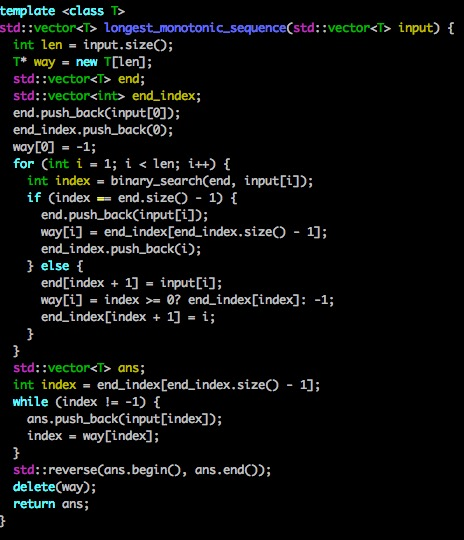
\includegraphics[height=4cm]{code}
  \label{pic:1}
\end{figure}

\subsection{实验效果}
下面是用\textit{test.py}脚本测试的概算的运行时间随着输入数据规模的增长图, 其中输入数据为随机生成的$[0, N * 0.4]$范围内的整数。




\end{document}
